Web Services sind aktuell die wichtigste Realisierung einer SOA und werden in der Software Industrie anerkannt. Mittlerweile setzen viele gro�e Softwarekonzerne auf Web Services und haben ihre Produktstrategien entsprechend ausgerichtet.

Als Web-Service bezeichnet man im Allgemeinen eine Softwarekomponente, die
ihre Funktionalit�at �uber Standardinternetprotokolle zur Verf�ugung stellt.
W3C definiert die Web Services folgenderma�en: 
\begin{Def}
A software application identified by a URI, whose interfaces and bindings are capable of being
defined, described, and discovered as XML artifacts. A Web service supports direct interactions
with other software agents using XML-based messages exchanged via Internet-based protocols.(W3C)
\end{Def}

a.) Ein Web Service wird durch einen URI identifiziert.1
b.) Die Schnittstelle eines Web Services ist maschinenlesbar und wird durch
WSDL (siehe n�chsten Abschnitt) beschrieben.
c.) Ein Web Service kommuniziert mit anderen Softwarekomponenten durch
XML Nachrichten. Der Nachrichtenaustausch kann insbesondere mit Hilfe
von Internetprotokollen (z.B. HTTP oder SMTP) stattfinden.

W�hrend die erste Definition die Eigenschaften von Web Services beschreibt,  die zweite Definition auf die wichtigen Standards ein. 
\begin{Def}
A Web service is a software system designed to support interoperable machine-to-machine
interaction over a network. It has an interface described in a machine-processable format
(specifically WSDL). Other systems interact with the Web service in a manner prescribed by its
description using SOAP messages, typically conveyed using HTTP with an XML serialization in
conjunction with other Web-related standards (W3C 2004a).
\end{Def}

Gem�� der beiden Definitionen sind die Beschreibung von Schnittstellen und
der Nachrichtenaustausch wesentliche Aufgaben. SOAP, WSDL und UDDI sind die daf�r vorgesehen Standards und bilden den Kern der Web Services.
\begin{itemize}
	\item SOAP ein standardisiertes, XML-basiertes
Protokoll zum Verpacken von Nachrichten, die zwischen Applikationen ausgetauscht
werden. setzt SOAP
auf die Netzwerk- und Transportschichten auf. Es ist also irrelevant, welche
Transportmechanismen f�ur den eigentlichen Versand verwendet werden.Die gebr�auchlichste Form des Austausches von SOAP-Nachrichten ist die �Ubertragung
�uber HTTP.
\item UDDI
dient zur Lokalisierung und Ver�ffentlichung
von Web-Services im Internet
UDDI = Register f�r Diensteund ihre Beschreibungen+ Suchmethoden+ Publishingmethoden
UDDI-Daten enthalten Kontakt-Informationen, Listen von Business Services und Infos, wie einService via Protokoll angesprochen werden kann
Um einen Web-Service im Internet zu finden, ist ein Verzeichnisdienst notwendig.
F�ur diese Zwecke wurde der Universal Description, Discovery and Integration-
Standard geschaffen. UDDI bietet Standardfunktionen zum Klassifizieren,
Katalogisieren und Verwalten von Daten und Metadaten �uber Web-
Services, so da� diese einfach gefunden und verwendet werden k�onnen.
\item WSDL (Web Services Defnition Language) ist eine funktionale, XML-basierte Beschreibungssprache
f�r die Schnittstellen eines Web Services.(siehe n�chsten Abschnitt)
\end{itemize}

\begin{figure}[htbp]
	\centering
		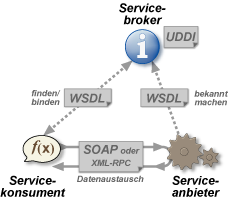
\includegraphics{bilder/Webservice.png}
		\caption{Kontrollfluss eines BPEL Prozesses}
	\label{fig:ExamlpleBPELProzess}
\end{figure}

Bei Web Services handelt es sich nicht um eine bestimmte Technik, sondern um ein B�ndel von verschiedenen Standards und Spezifikationen.
Web Service Stack ...

Bild

Im n�chsten Abschnitt wird WSDL etwas genauer vorgestellt.

